\clearpage

\section{Entropy Estimator}

\begin{tcolorbox}	
\begin{tabular}{p{2.75cm} p{0.2cm} p{10.5cm}} 	
\textbf{Header File}   &:& entropy\_estimator\_*.h \\
\textbf{Source File}   &:& entropy\_estimator\_*.cpp \\
\textbf{Version}       &:& 20180621 (MarinaJordao)
\end{tabular}
\end{tcolorbox}

\subsection*{Input Parameters}

The block accepts one input signal,a binary, and it produces an output signal with the entropy value.
No input variables in this block.


\subsection*{Functional Description}


This block calculates the entropy of a binary source code composed 0 and 1.
\subsection*{Input Signals}

\textbf{Number}: 1\\
\textbf{Type}: Binary

\subsection*{Output Signals}

\textbf{Number}: 1\\
\textbf{Type}: Real (TimeContinuousAmplitudeContinuousReal)
%\end{document}


\clearpage

\section{Entropy Estimator}

\maketitle


\subsection*{Functional Description}
\paragraph{}
entropyEst(vector$<$Signal *$>$ \&InputSig, int window)
\paragraph{}
The estimator sweeps the full range of the binary input computing an entropy estimation for each window. Then, the entropy mean, the variance and the individual entropy estimations are outputted to a file.

\subsection*{Input Parameters}
\paragraph{}
The block accepts as input parameter the window size, which defines the length over which each entropy estimation is computed.

\paragraph{}
Note: If the length of the binary stream is not an integer multiple of the window size, the estimator considers the window size equal to the full length of the input signal.


\subsection*{Input Signals}

\textbf{Number}: 1

\textbf{Type}: Binary Stream

\subsection*{Output Data}
\paragraph{}
Entropy mean, entropy variance and entropy estimations.

\paragraph{}

The entropy estimator generates a file with the name \texttt{"entropy\_est.txt"} where the output data is written.

\begin{figure}[H]
\subsection*{Results}
    \centerline{
       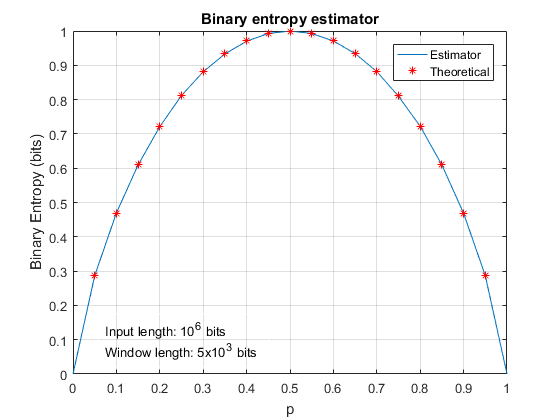
\includegraphics[scale=0.75]{./lib/entropy_estimator/figures/BinEntropyResults.png}
    }
\end{figure}

